\section{Data analysis}

Three software packages were used for data preprocessing: Elekta Neuromag\textsuperscript{\textregistered} MaxFilter (version 2.2, \cite{3.3.MNE}), Matlab (version 2014a) and MNE-Python (version 0.8.6, \cite{3.3.MNEpython}).

\subsection{Behavioral data}

Two types of behavioral data were analyzed for group and condition effects: response time (RT) and response accuracy (RA).
Response time was measured at the condition onset, i.e. at the ``d`` sound of ``den`` or ``der`` (in the subject-relative clause or the object-relative clause, respectively).
Trials were omitted when the subject skipped or answered them incorrectly.
Trials were also omitted if the response took longer than 4000ms.
This procedure removed 11.1\% of the childrens' trials, and 2.5\% of the adults' trials.

RT and RA were determined for each subject separately from the remaining trials.
Both metrics were tested for the requirements for an analysis of variance (ANOVA).
Normality of the residuals was tested with a Shapiro-Wilk test \cite{3.3.swtest}, implemented in Matlab.
Equality of variances was tested with a Levene test\cite{3.3.levtest}, implemented in SPSS.
RA data failed the normality test.
To include RA data in the following analysis, they were transformed to fit a normal distribution.
This transformation was accomplished with the inverted sigmoid function:
\[ \hat{a} = - log( \frac{1}{a} - 1 ) \]
All results from the ANOVA were transformed back into milisecond space with the sigmoid function:
\[ r = \frac{1}{1+e^{-\hat{r}}} \]

\subsection{Sensor-space activity}

\paragraph{Preprocessing and HPI correction}
Signal-space separation \cite{3.3.SSS} was used to reduce noise in the data by suppressing magnetic interference coming from outside and inside the sensory array.
MEG recordings were corrected for HPI movements, and co-registered across blocks to the inital head position for each individual.
All of these steps were computed with MaxFilter.
Data were then subjected to a FIR highpass filter (Hamming window design, 4367 coefficients, -130dB suppression at 0Hz, 3dB breakpoint at 0.5Hz, processing in Matlab) to remove slow trends.

\paragraph{Artifact removal}
MEG channels with abnormally high noise levels as identified by visual inspection were rejected from further analysis. A median of 1 channel (maximum: 3 channels) was removed.
The resulting pre-processed data contained major artifacts from spontaneous channel jumps, electrocardiographic (ECG) activity and electrooculographic (EOG) activity.
Jump amplitudes were detected by selecting peaks in the z-transformed continuous data that exceeded a threshold of 12 standard deviations.
Segments of 2 seconds in the pre-processed continuous data were rejected if any magnitude channel exceeded an amplitude of $6\cdot10^{-12}T$ (gradiometer channels: $4\cdot10^{-12}\frac{T}{cm}$).
Continuous data were then decomposed into independent components (ICA) that explained 99\% of the variance.
Components that correlated with EOG or ECG channels were removed with the MNE functions \emph{preprocessing.ica\_find\_ecg\_events} and \emph{preprocessing.ica\_find\_eog\_events}, respectively.
ICA-based correction removed an average of 2.1 components per subject and block (minimum: 1, maximum: 4).
The remaining ICA components were used to reconstruct continuous data.

\paragraph{Epoching}
The main trigger was set at the condition onset (described in section 3.1.4).
Epochs were created between 1000ms before and 4000ms after the main trigger.
An epoch was rejected if the trial was skipped, or answered too slow (more than 4000ms) or answered incorrectly.
This procedure yielded an average of 274 (90\%) trials in children and 297 (98\%) trials in adults.
Data were filtered before epoching with a 45Hz FIR lowpass (using the MNE function \emph{raw.filter}) exclusively for the following two steps.

\paragraph{Cluster analysis}
Each trial consisted of mean activity from one of each of three sensor groups (from parietal, temporal and frontal locations).
Trials from each syntax condition were pooled into a pair of trial sets.
Since the group had a strong impact on RT (see section \ref{results}), effective time windows were estimated separately for children and adults.
Clusters were computed by running the MNE function \emph{stats.permutation\_cluster\_test} \cite{3.3.clustertest} with the pair of trial sets as input data.
The function was run with 2500 permutations, and an t-threshold of 2.0.

\paragraph{Interval analysis}
Additionally, a blind comparison was performed for sensor activity in a series of time intervals.
10 time intervals were established from 0ms to 2200ms\footnote{As determined in the following analysis of response times, these intervals cover 95\% of childrens' trials completely, and 98\% of the adults'.} after onset, spanning 200ms each.
The mean sensor activity was computed for each sensor group (3), hemisphere (2), time interval (10), yielding 60 activity values for each subject and condition.
The corresponding values were pooled over all subjects within each of the two groups, and compared between syntax conditions with a paired Student's T-test.
Results from each hemisphere and sensor group were adjusted with the false discovery rate correction (10 comparisons).

For visualization purposes, grand average activity was also calculated for each sensor group and condition, separately for children and adults.

\begin{figure}[h]
\begin{center}
\vspace{7mm}
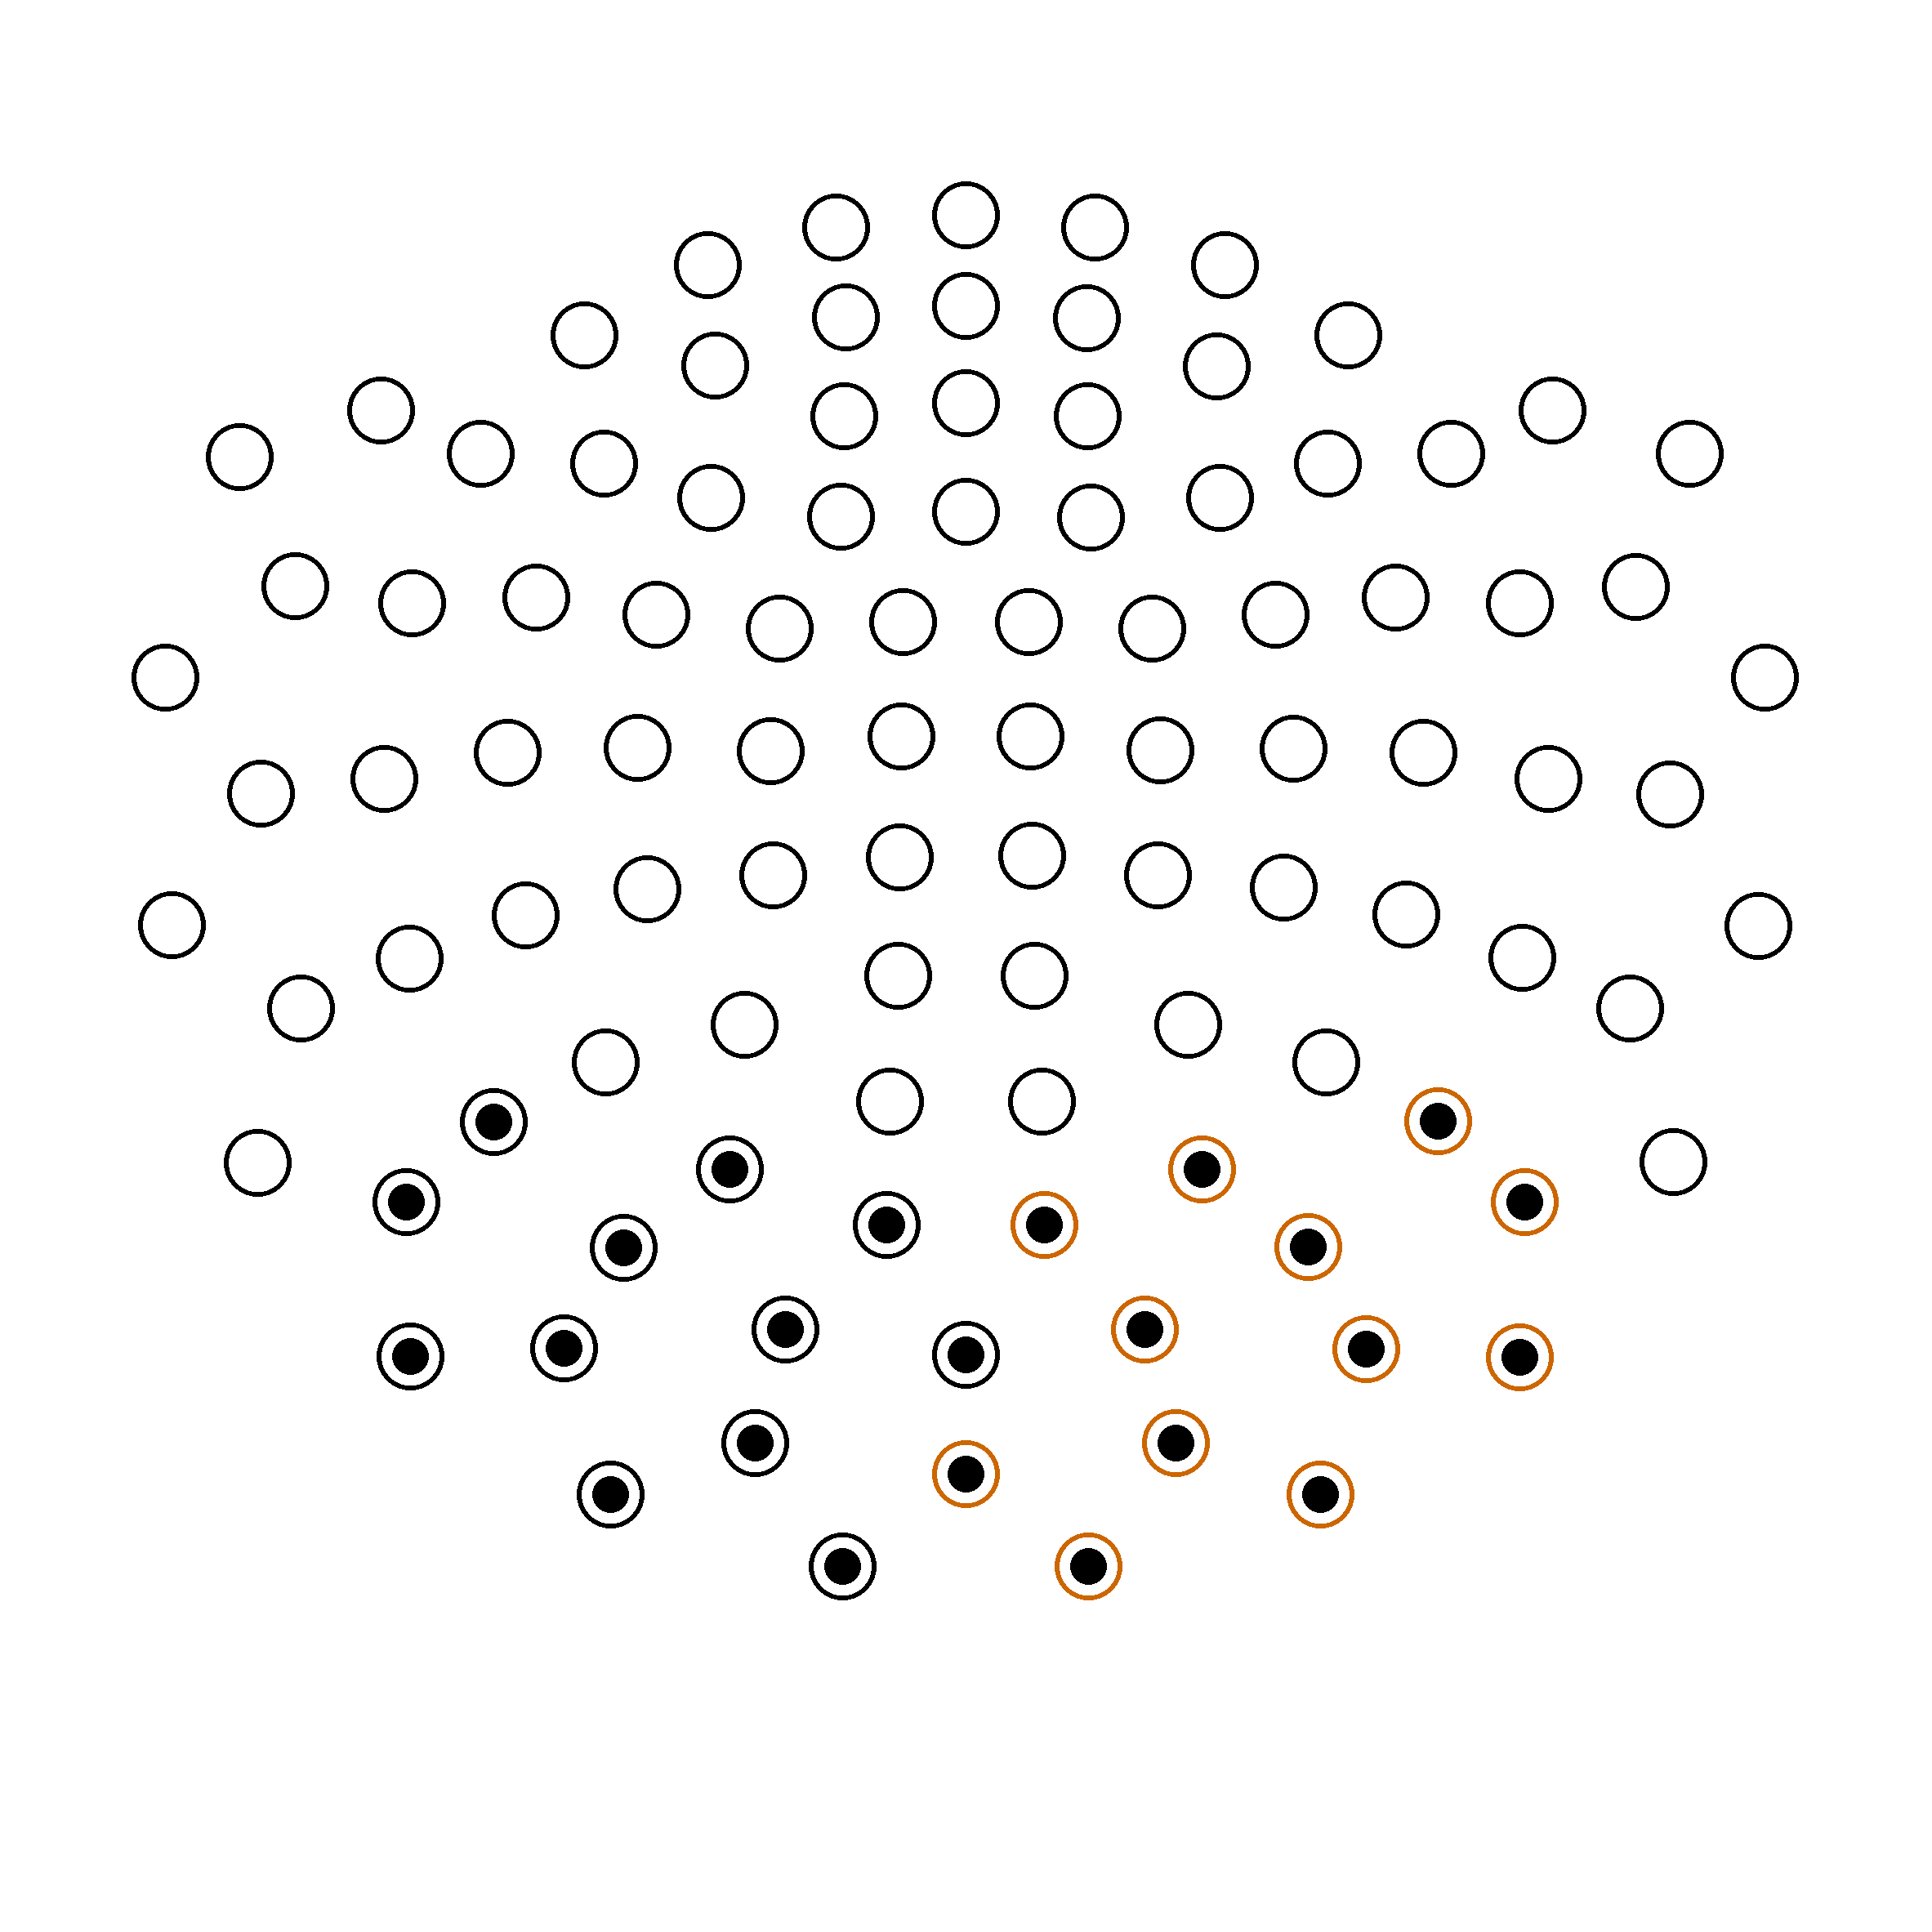
\includegraphics[width=0.24\textwidth]{pics/3_3_occipital_sensors}
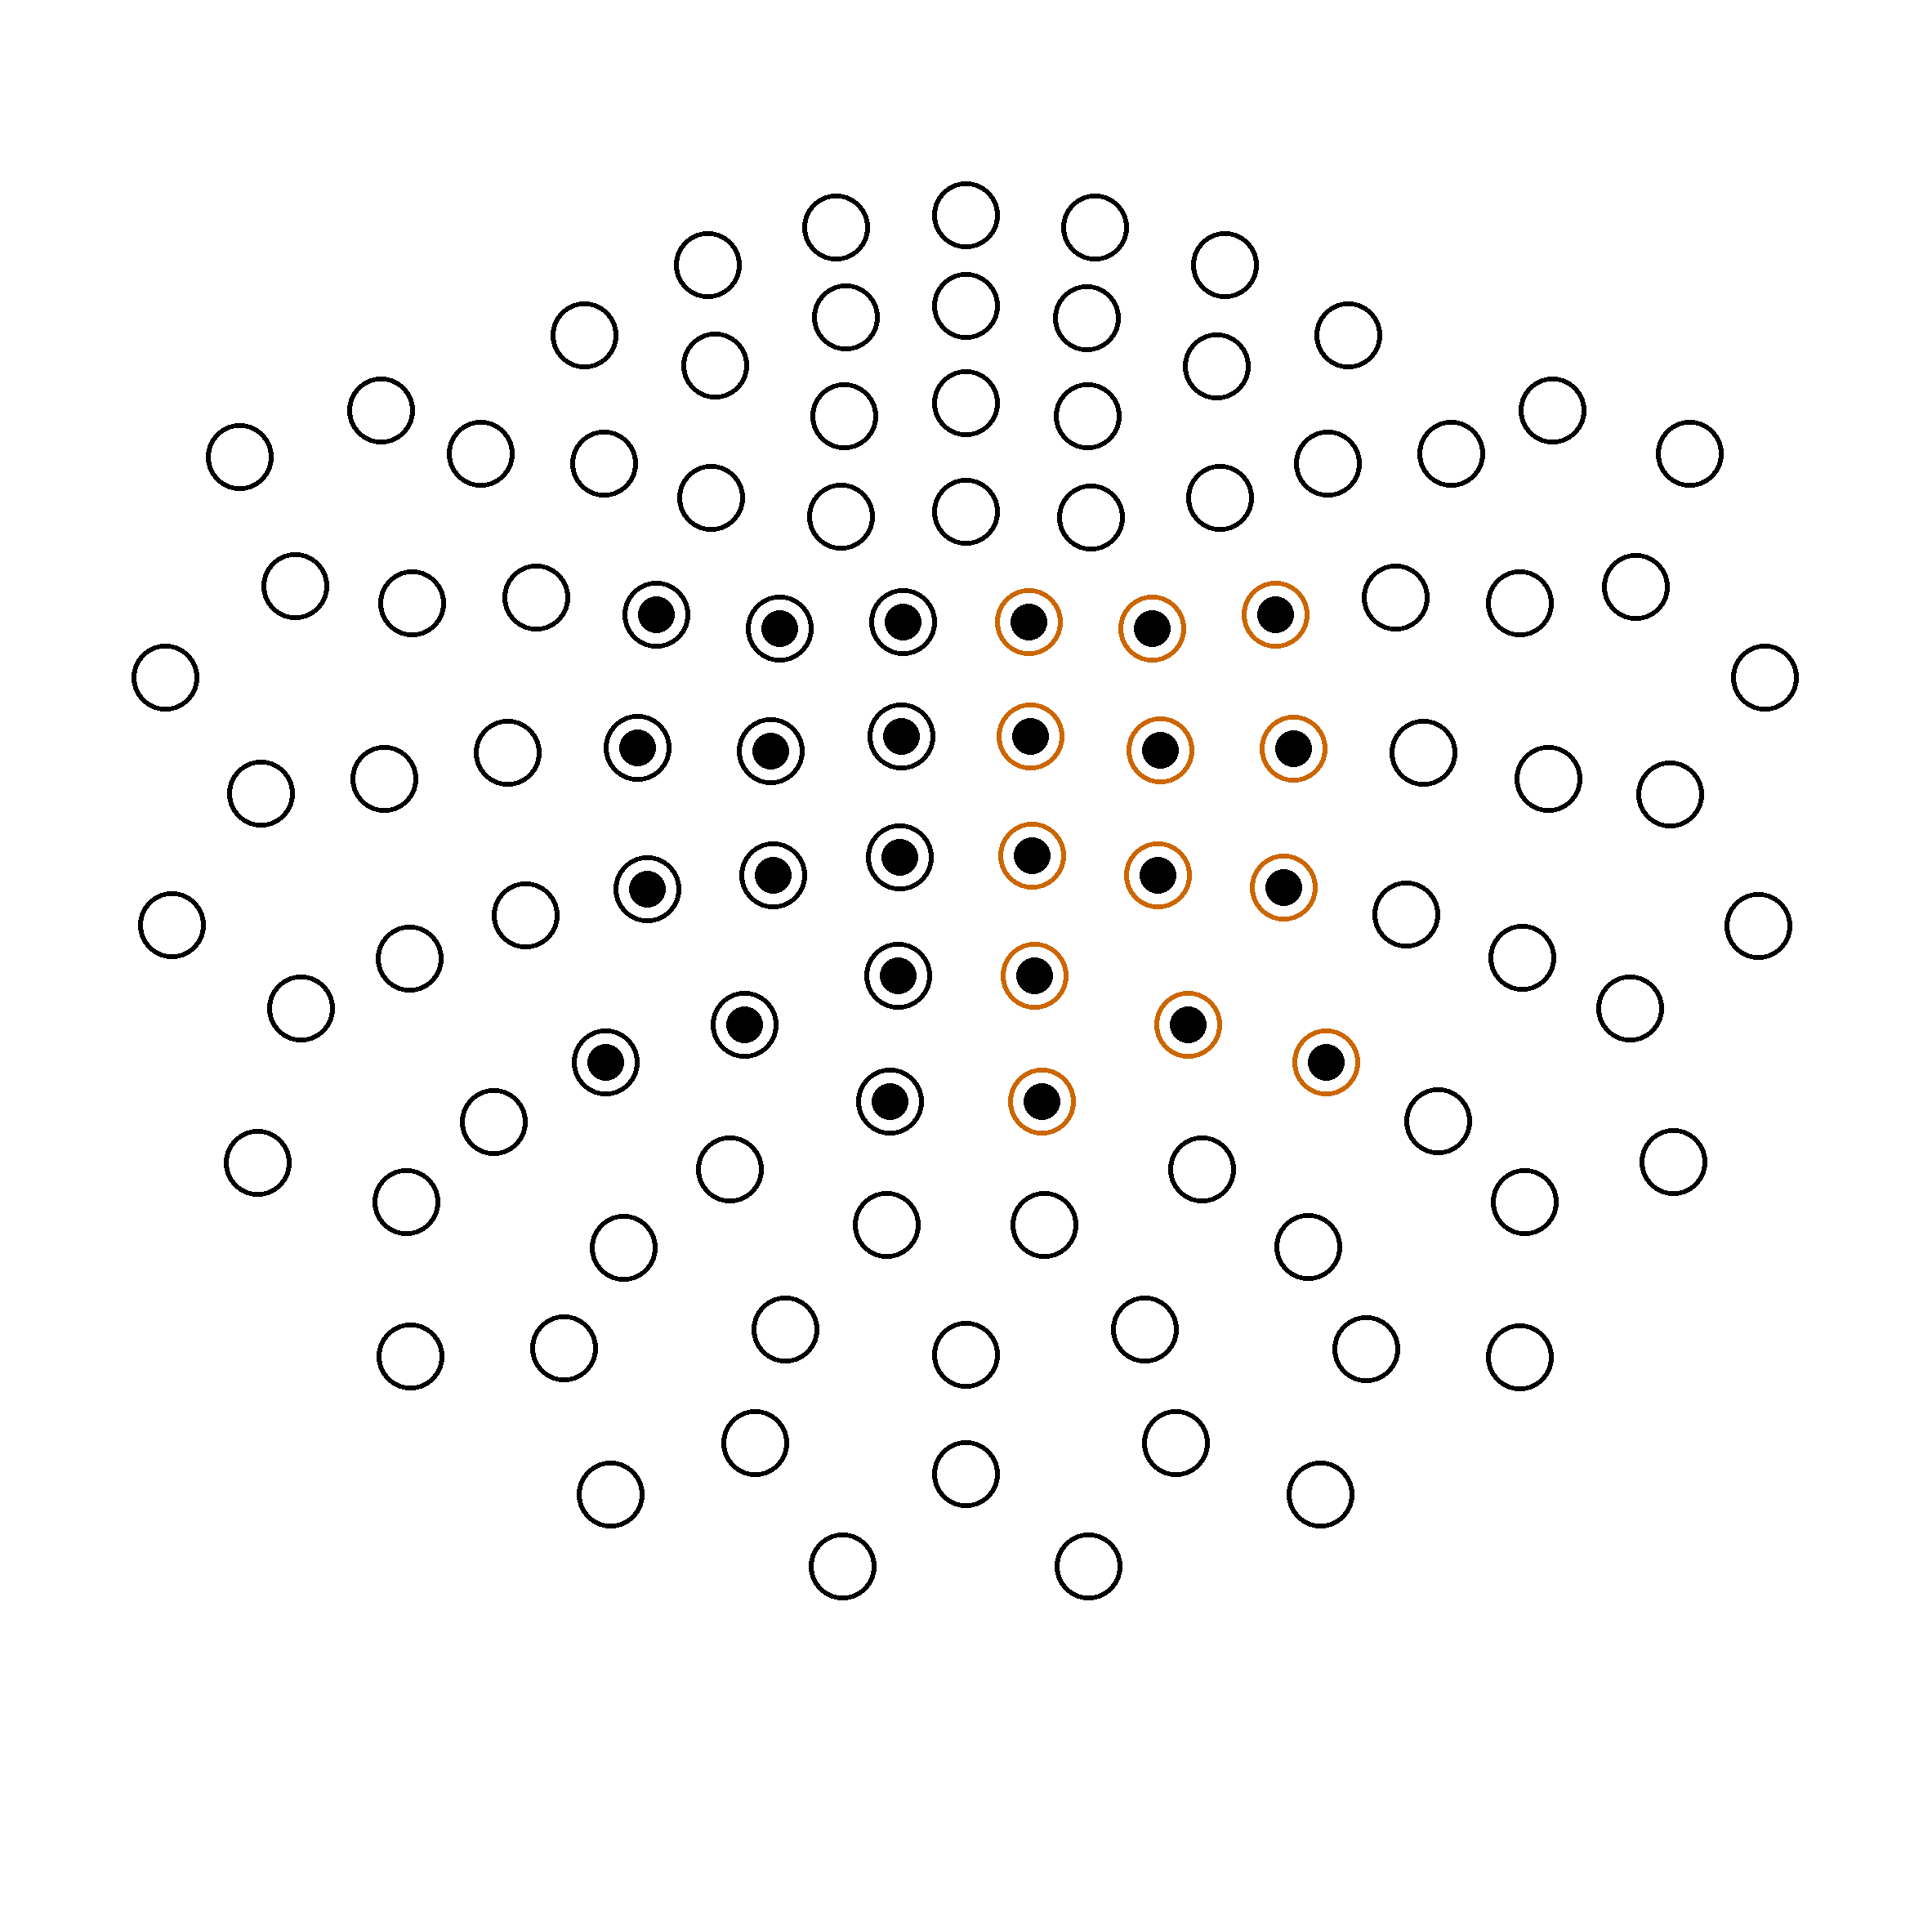
\includegraphics[width=0.24\textwidth]{pics/3_3_parietal_sensors}
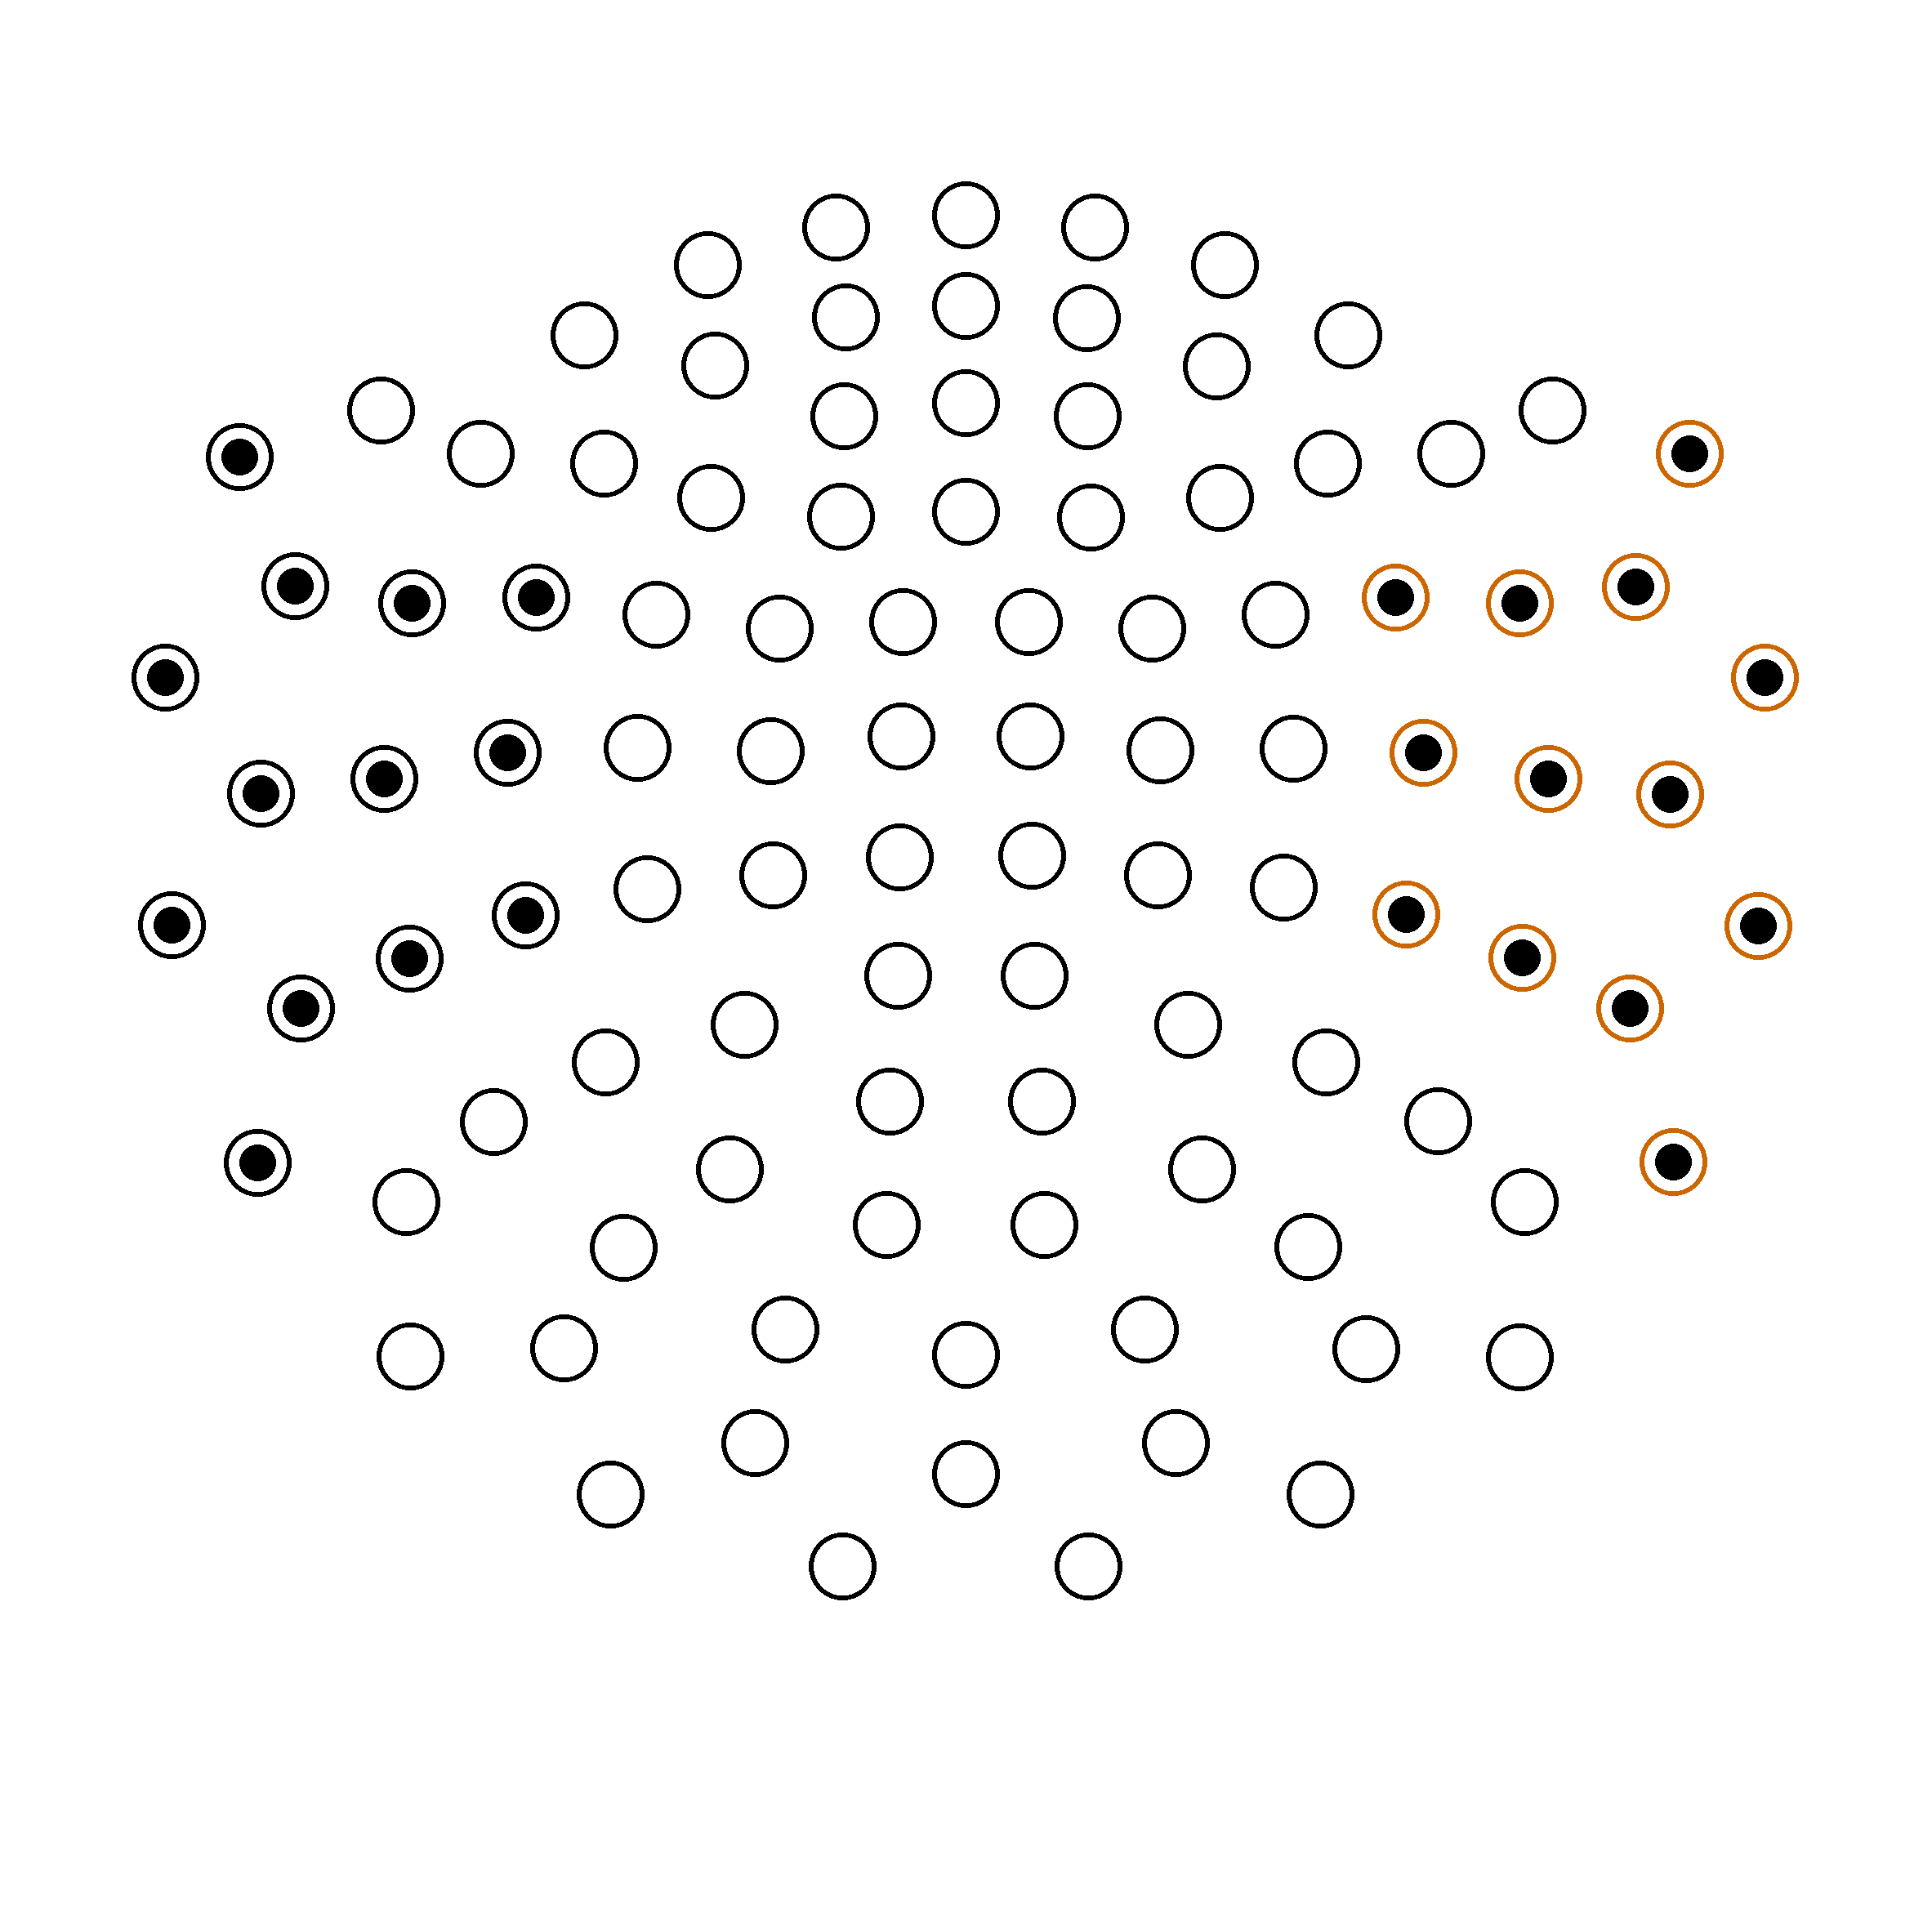
\includegraphics[width=0.24\textwidth]{pics/3_3_temporal_sensors}
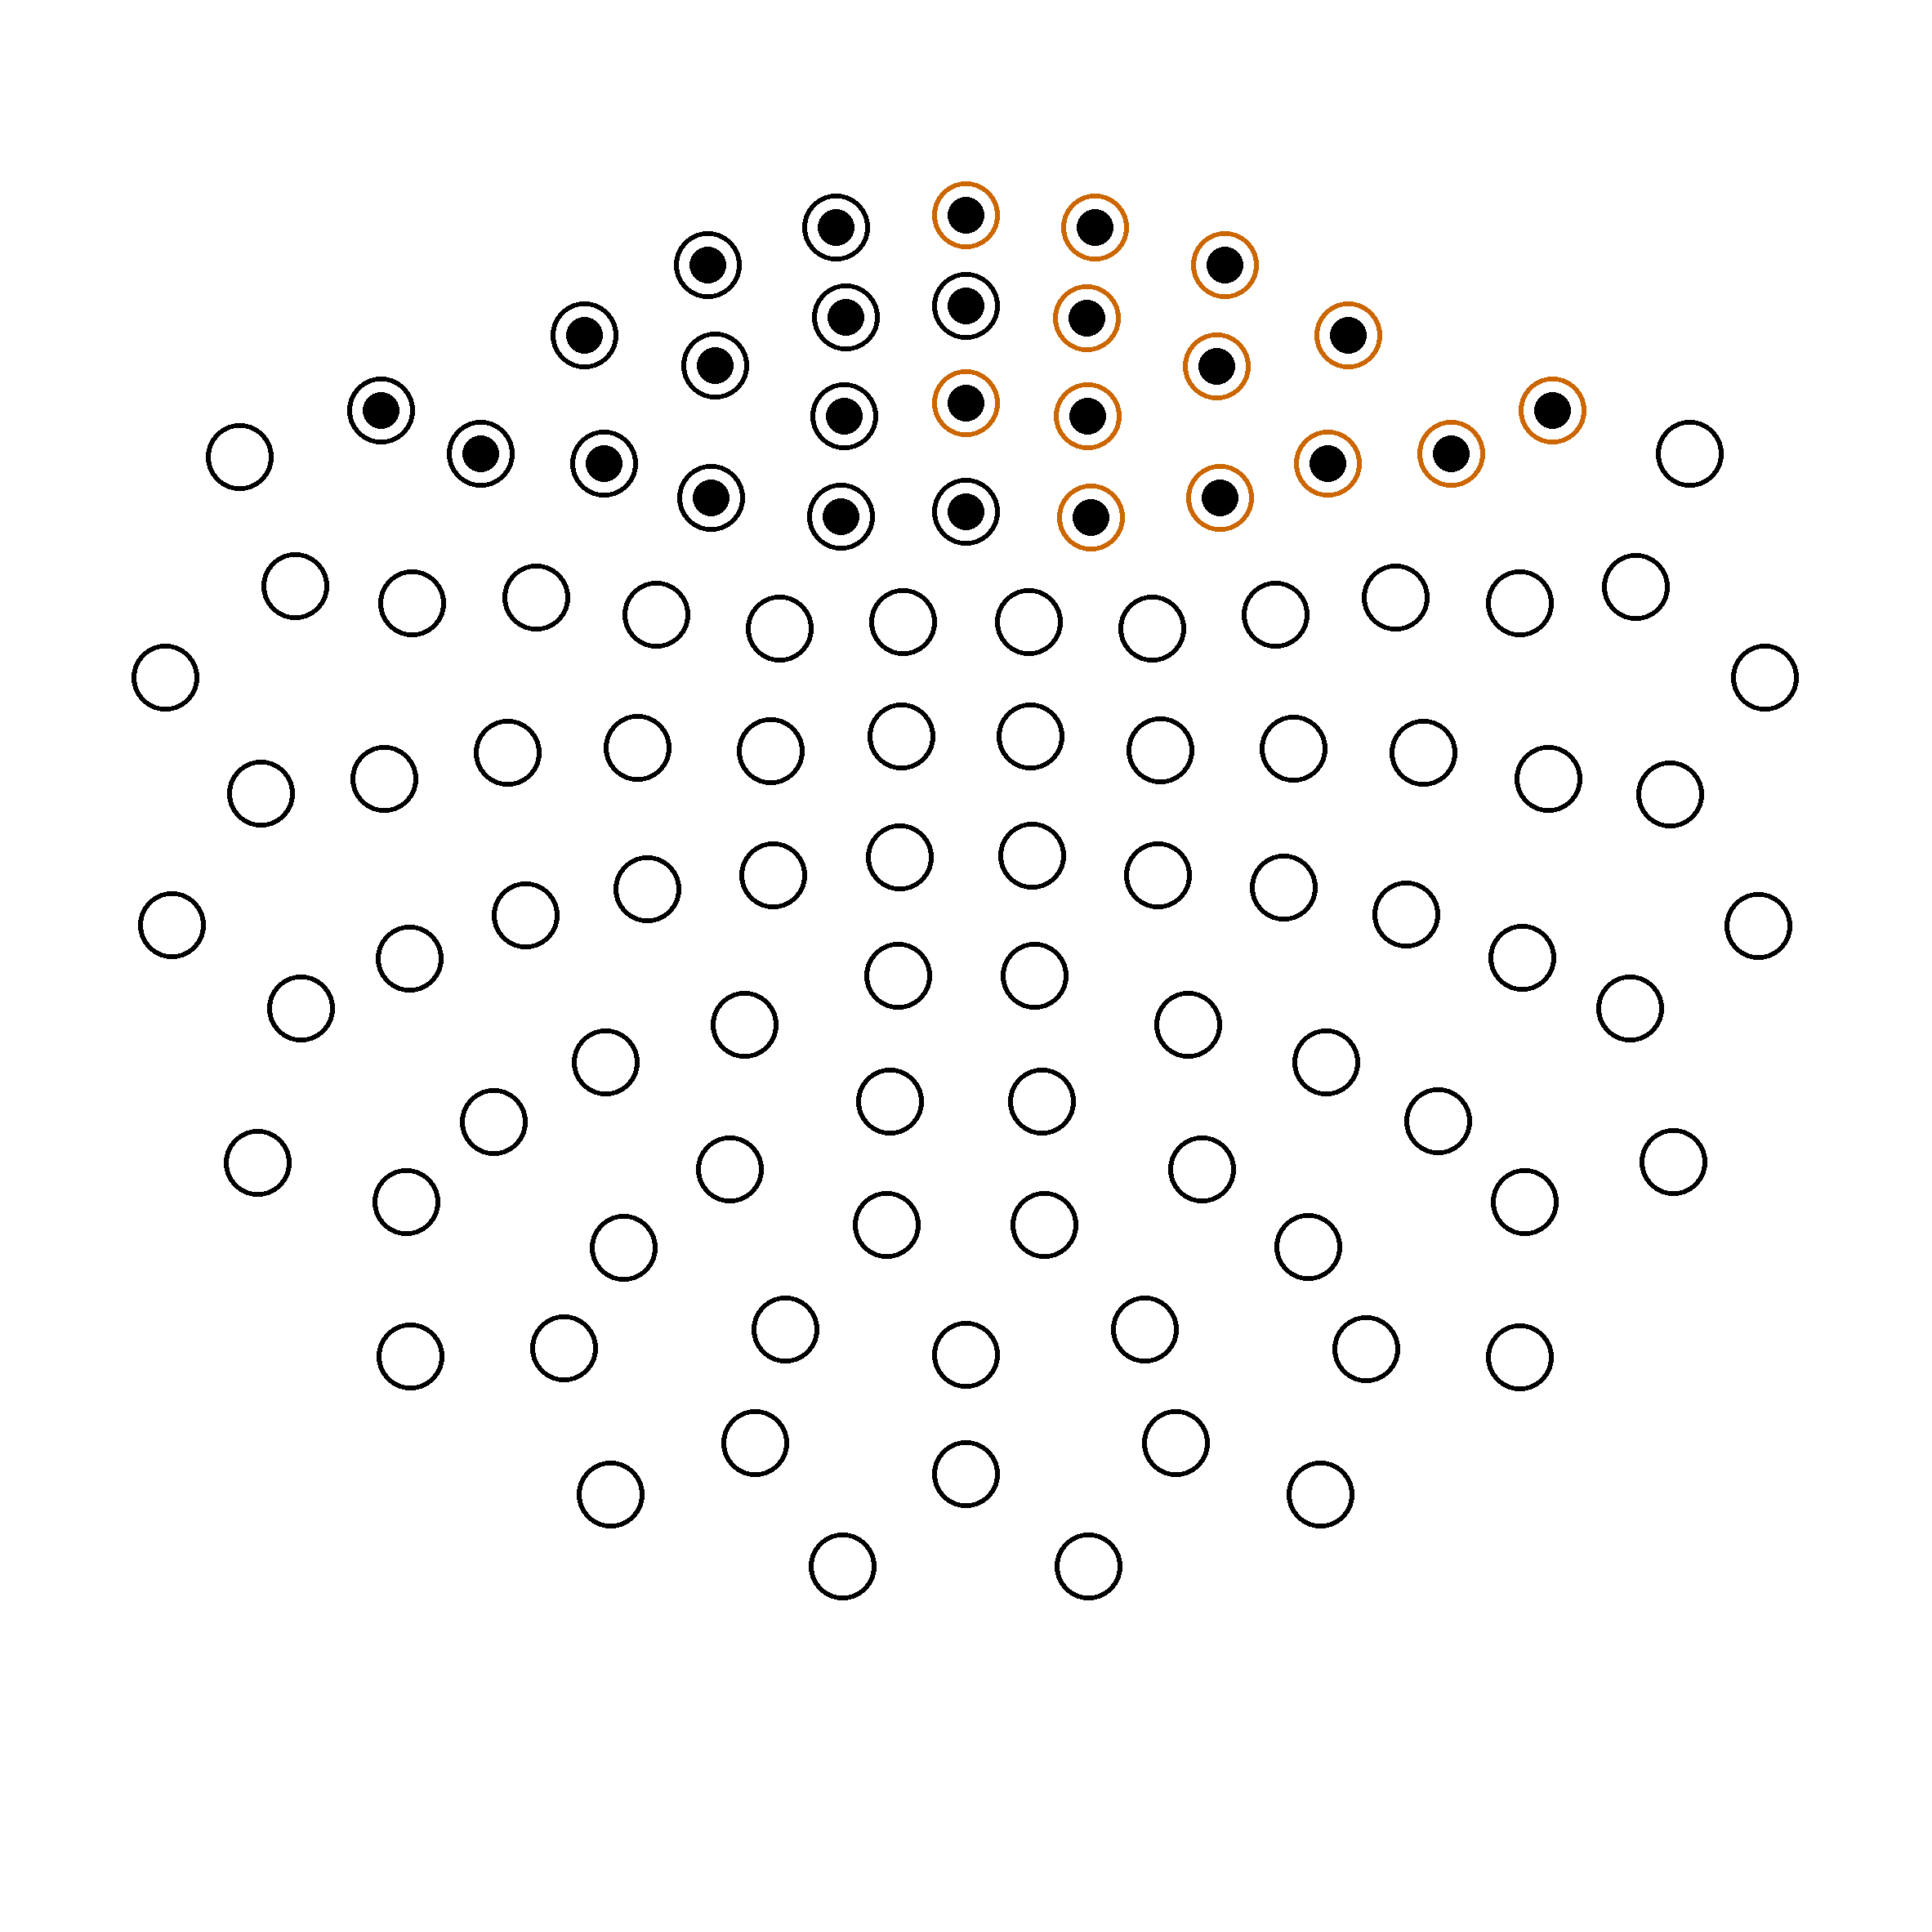
\includegraphics[width=0.24\textwidth]{pics/3_3_frontal_sensors}
\caption{\label{3.3.sensors} Selected channels for each sensor location. From left to right: occipital, parietal, temporal, frontal. The right hemisphere (in red) is also depicted on the right side in each illustration.}
\end{center}
\end{figure}

\subsection{Source space activity}

\paragraph{Anatomical preprocessing}
Cortical reconstruction and volumetric segmentation was performed with the Freesurfer image analysis suite [Martinos Center for Biomedical Imaging, Harvard-MIT, Boston USA].
I followed the recommended processing pipeline (``recon-all``), with three optional functions.

First, the option ``-nuintensitycor-3T`` improved brain segmentation accuracy by optimizing the bias field correction \cite{3.3.nuintensity}.

Second, by invoking ``-notal-check``, I skipped the Talairach registration checks.
Talairach registration was prone to failure especially in the infant subjects, and uneccessary for our further processing steps.

Third, I supplied and included T2-weighted MRI datasets with the options ``-T2`` and ``-T2pial``.
The combination of T1- and T2-weighted images improves tissue differentiation especially around the pia mater, yielding a more accurate cortex segmentation.
This pipeline yielded a continuous, antomically plausible cortical surface in MRI space.


\paragraph{Forward and inverse operator}
For the forward operator, three components were necessary: a source model, a BEM model and a coregistration file.

The cortical surface from Freesurfer was used to construct the source model.
Sources were generated by the MNE package \emph{mne\_setup\_bem}.
The result were 20484 sources (10242 per hemisphere), distributed with approximately equal density over the cortical surface.

The head surface from Freesurfer was used to extract a scalp surface layer.
The BEM was constructed from this scalp layer with the MNE package \emph{mne\_surf2bem}, using the default options.
This function sampled down the original surface to the 4th subdivision of an icosahedron.
The finished BEM consisted of 5140 nodes.

Finally, a coregistration file provided the transformation between MRI space and MEG space.
This coregistration attempted to minimize the distance between digitized head surface points and the head surface extracted from the MRI. 
It was performed for each subject individually using the MNE package \emph{mne\_analyze}.
The initial fit was done manually, with visual error feedback.
The following fine adjustment was performed automatically.
This process was repeated until the average spatial error was less than 2mm.
These three components were assembled into a forward operator by the method \emph{mne\_do\_forward\_solution}.


For the inverse operator, three components were necessary: the forward model, a noise covariance matrix, and a regularization factor.
Each component was calculated individually for each subject.

The first component, the forward model, was supplied by the previous step.

For the second component, the noise covariance matrix, the 1000ms after visual onset were extracted from each trial.
Then, the covariance matrix was computed from this data with the function \emph{mne.compute\_covariance}.

The third component, the regularization factor was determined from this noise covariance matrix.
First, only coefficients from gradiometer channels were selected.
Second, these coefficients were transformed with a singular value decomposition.
Third, the upper cutoff was defined as the first value of the transformed coefficients.
Fourth, the index at which the transformed coefficients performed the steepest drop in logarithmic value was determined.
Fifth, this index was defined as the maximum amount of usable dimensions.
Sixth, the lower cutoff was defined as the value at this index, plus 15\%.
Seventh, the regularization factor was computed by dividing the lower cutoff by the higher cutoff.


The inverse operator was computed from these three components by the method \linebreak \emph{mne\_do\_inverse\_operator}.
The regularization factor was supplied with the option \linebreak ``--megreg``.

\paragraph{Inverse solution}
For determining regional cortical activity, 8 regions needed to be defined: the primary auditory cortex (PAC), the anterior and posterior parts of the superior temporal sulcus and gyrus (aSTS, pSTS, aSTG and pSTG), Brodmann area 45 (BA45), Brodmann area 44 (BA44) and the ventral Brodmann area 6 (BA6v).
These regions were spatially defined manually on the cortex of the reference subject.
Freesurfer provided the aparc.a2009s segmentation, which became the basis for this regional selection.
The final regions of interest on the reference brain are visualized in Fig. \ref{3.3.ROI}.
Regions were then mapped from the reference cortex onto the cortices of all other subjects during the next step.

\begin{figure}[h]
\begin{center}
\vspace{7mm}
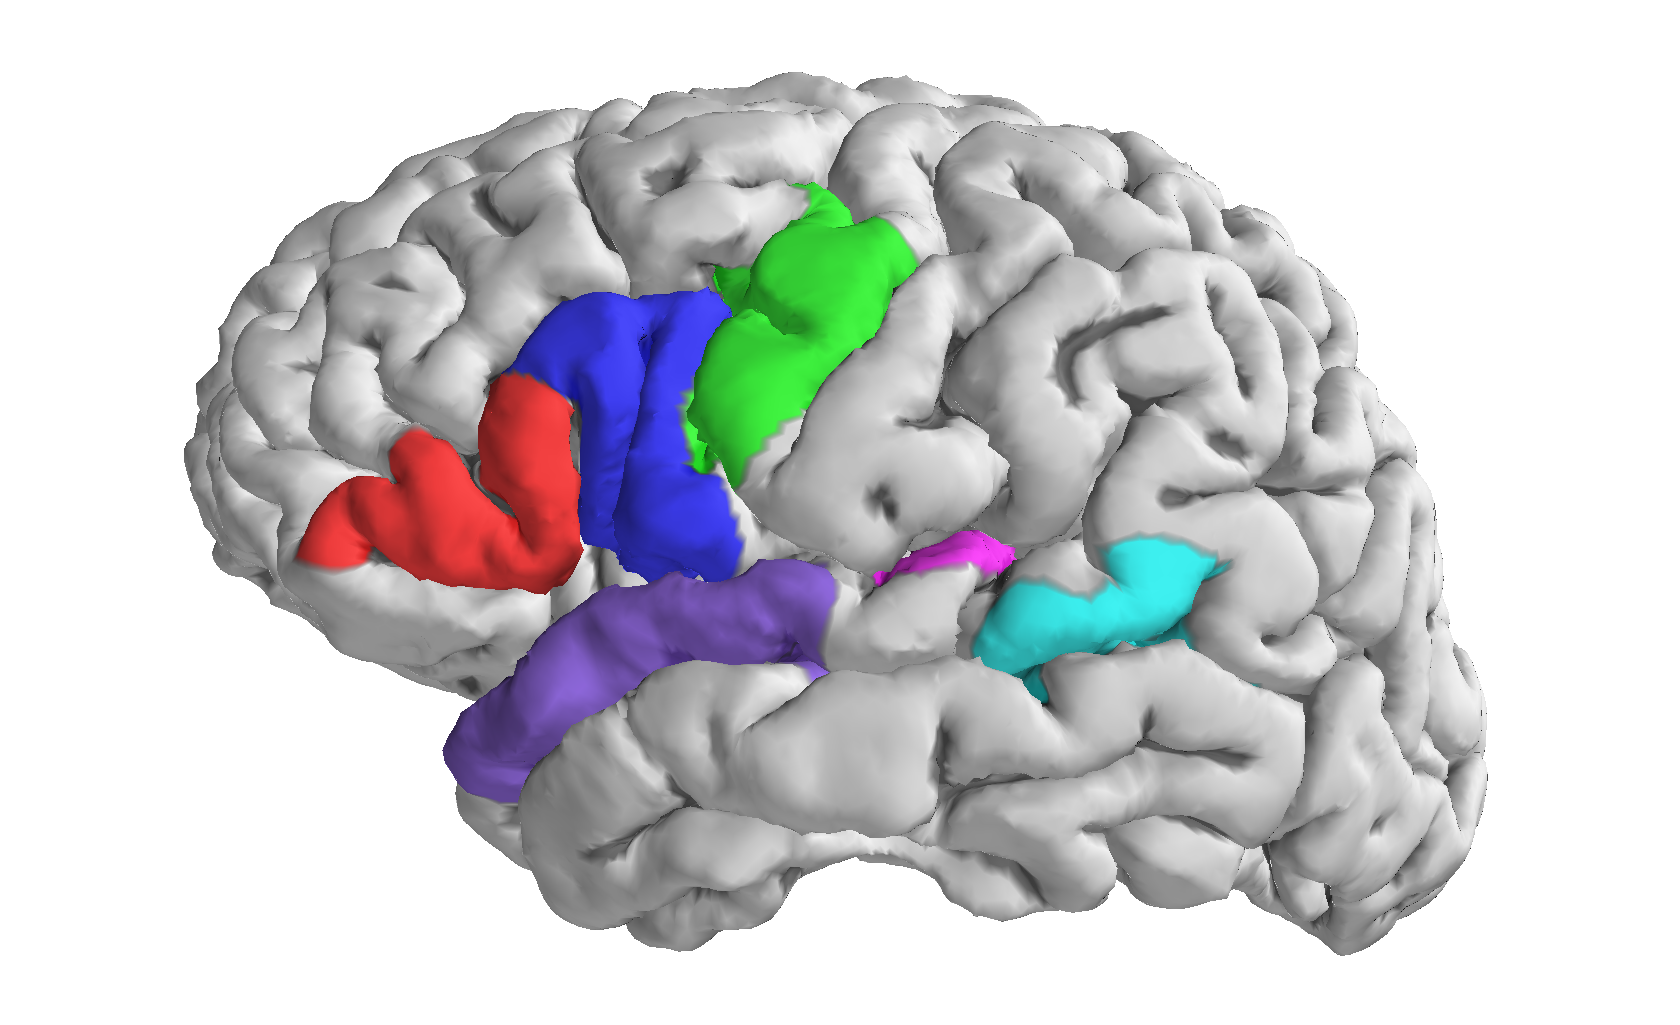
\includegraphics[width=0.49\textwidth]{pics/dh55a-pial-lh}
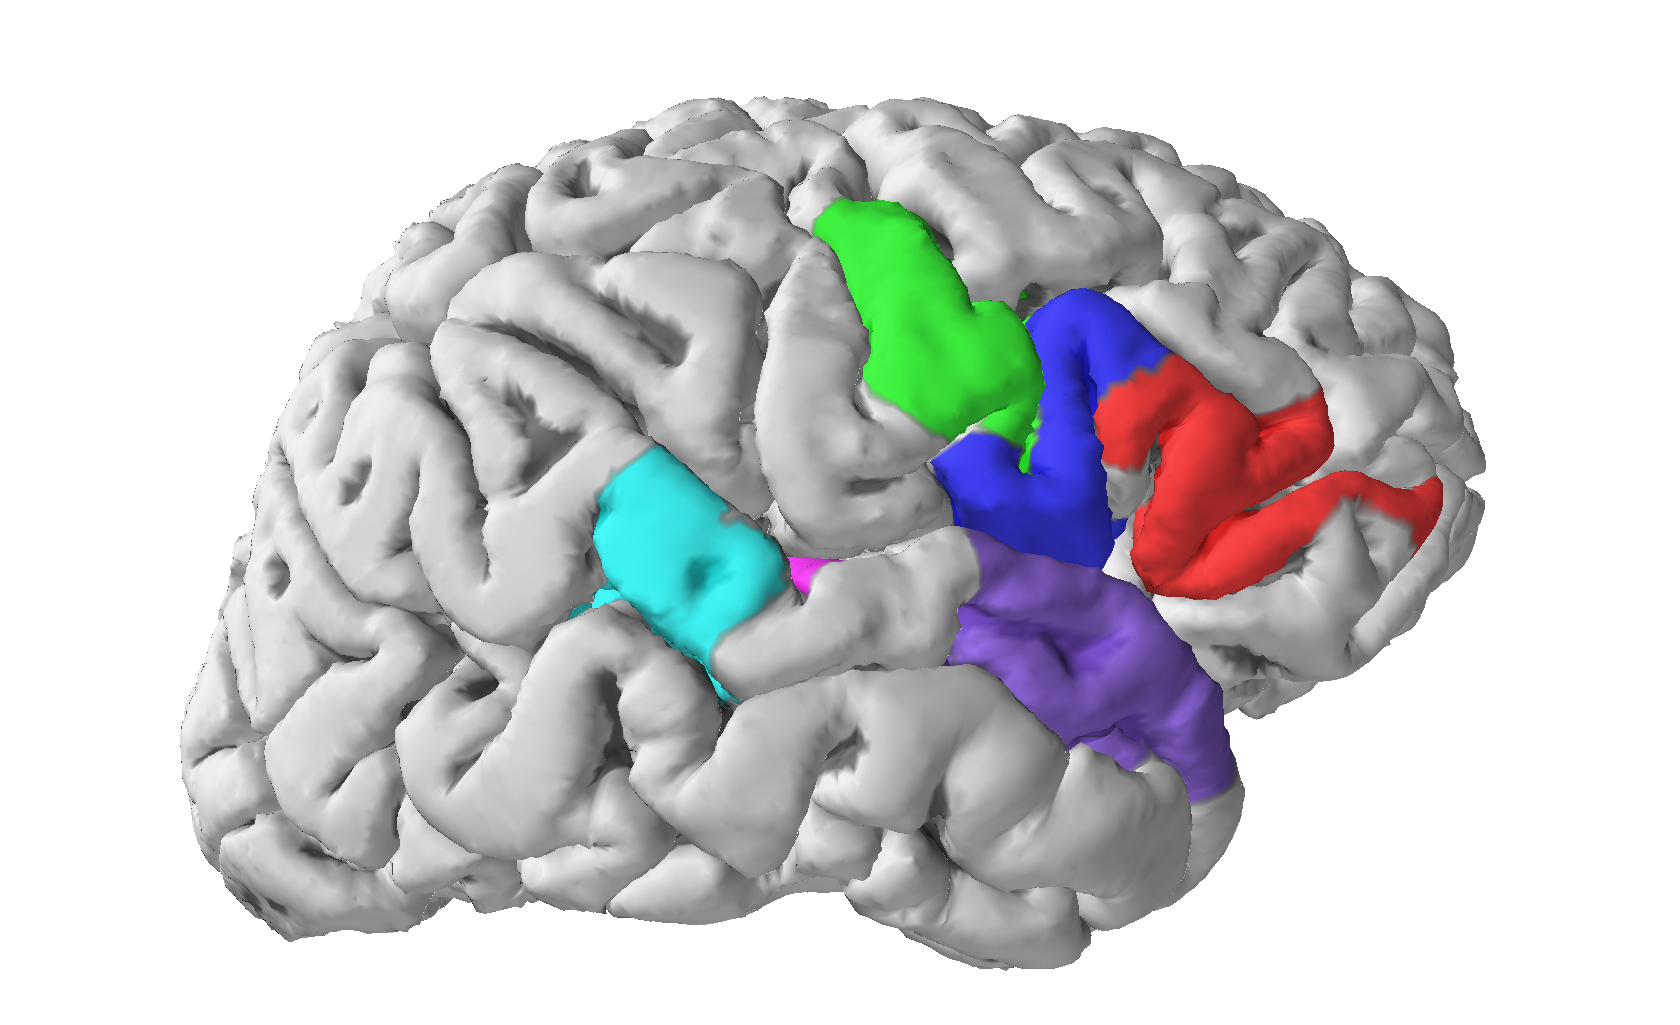
\includegraphics[width=0.49\textwidth]{pics/dh55a-pial-rh}
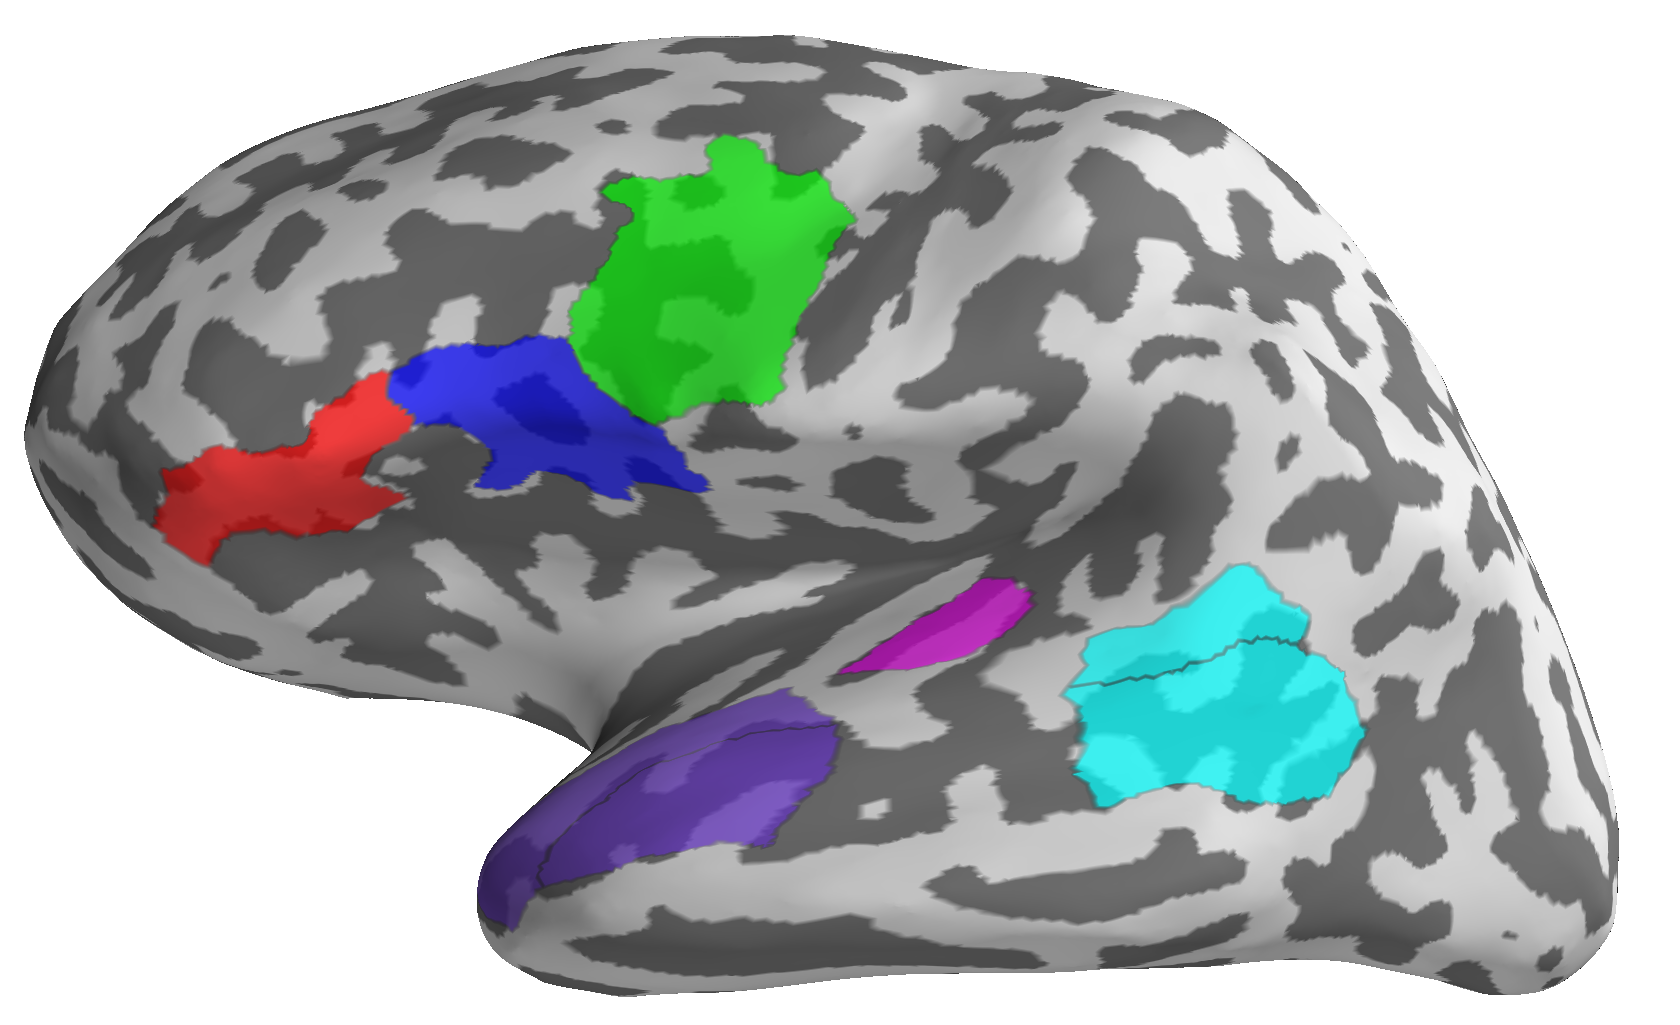
\includegraphics[width=0.49\textwidth]{pics/dh55a-inflated-lh}
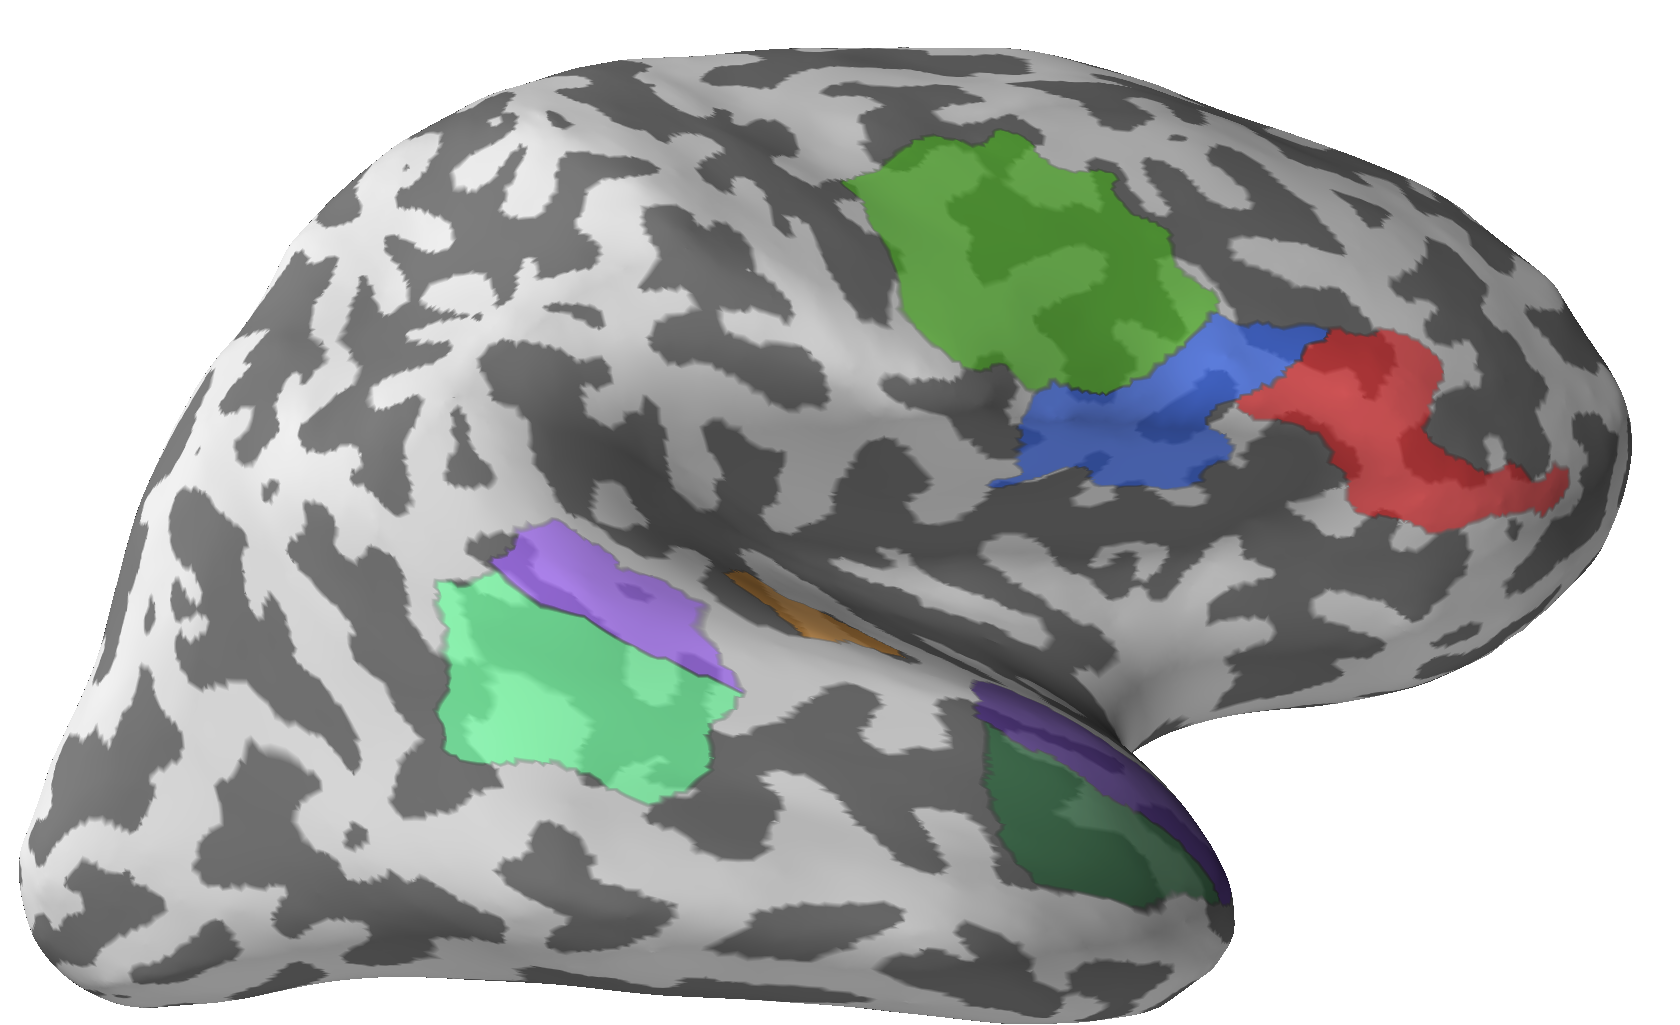
\includegraphics[width=0.49\textwidth]{pics/dh55a-inflated-rh}
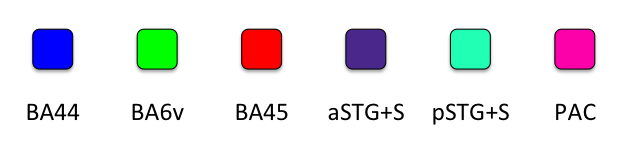
\includegraphics[width=0.75\textwidth]{pics/3_3_ROIlegend}
\caption{\label{3.3.ROI} Selected regions of interest on the reference brain. Top: selected regions on the folded cortex. Bottom: selected regions on the inflated cortex.}
\end{center}
\end{figure}

The inverse operator was then used to calculate inverse solutions from MEG sensor data.
Inverse solutions were calculated for each time point, region, trial and subject individually.
The process was performed by the function \emph{mne.minimum\_norm.apply\_inverse\_epochs}, with sLORETA as the inverse method.
The option ``pick\_ori=normal`` designated currents leaving and entering the cortex as positive and negative, respectively.
Due to the combination of passive and active noise reduction and artifact suppression, I assumed a fairly high signal-to-noise-ratio (SNR) of 50:1 for each individual source.
The regularization factor was estimated by $\frac{1}{SNR} = 2.5*10^{-3}$.
The result was a series of activation patterns within each region.
Finally, the mean of regional node activity was calculated for each time point, region, trial and subject.

The resulting localized activity was subjected to a cluster analysis.
Extracted trials were pooled over all subjects within a group.
Within each group, two sets of trials were created from the two syntax conditions.
Each trial contained mean activity from eight regions (PAC, aSTS, aSTG, pSTS, pSTG, BA44, BA45 and BA6v).
Clusters were determined by running the MNE function \emph{stats.permutation\_cluster\_test} \cite{3.3.clustertest} over the two sets of trials.
The function was run with 2500 permutations, and an t-threshold of 2.0.
The results from each group was evaluated separately.

Additionally, a blind comparison was performed for sensor activity in a series of time intervals.
10 time intervals were established from 0ms to 2200ms after onset, spanning 200ms each.
The mean activity was computed for each region (8), hemisphere (2), and time interval (10), yielding 160 activity values for each subject and condition.
The corresponding values were pooled over all subjects within each of the two groups, and compared between syntax conditions with a paired Student's T-test.
Results from each hemisphere and region were adjusted with the false discovery rate correction (10 comparisons).

For visualization purposes, grand average activity was calculated for each cortical region, group and condition.